% Proposal

\chapter{Proposal} % Main chapter title

\label{Proposal} % For referencing the chapter elsewhere, use \ref{Chapter1} 

\lhead{Chapter 4. \emph{Proposal}} % This is for the header on each page - perhaps a shortened title

In this chapter, we would introduce our proposal and contribution to current VLC researches. 

%----------------------------------------------------------------------------------------
%	HARDWARE
%----------------------------------------------------------------------------------------

\section{System Description}


Considering previous results and solutions, we propose an innovative solution, taking advantage of the Ara modular smartphone,
to design a well suited front-end receiver for visible light communication.

As the Ara platform let use choose our own hardware and receiver, we would avoid problems and sampling limitations related to camera, or ambient light sensor.
On other hand, the modular platform, through its UniPro interface on the endoskeleton board, give us the possibility to connect our module with the same performance than if it has been directly pluged in the main application processor board.
In this way, we don't need to use a smartphone peripheral, such as USB, or Bluetooth controller, that would add a huge overhead in the transmission and processing.

The system, that we develop as part of this project consist in a commercial LED emitter, driven by a STM32L0 micro-controller unit, in order to transmit the OOK modulated signal. Before that, we propose to encode data using 4B6B or Manchester, in order to perform different experimentation and compare the result.

Considering the receiver module, our light sensor consist in a photodiode followed by several electronic circuit : current to tension converter, low-pass filter and positive gain amplifier.

The analog to digital conversion has been realized at 1,1 MSPS by the micro-controller unit. To fit the platform requirement and optimize the throughput, it performs several operations such as thresholding, decoding and buffering.

The transmission between the MCU and the Ara Development Kit is achieved through I2C bus in "slave-transmit" mode, with the MCU as slave-node and the ARA as master-node.

Finally, we develop a basic Android application for the platform, that implement I2C bus initialization, data polling, and logging for later computation and analysis.

\begin{figure}[htbp]
  \centering
    \makebox[\textwidth][c]{
      \scalebox{0.4}{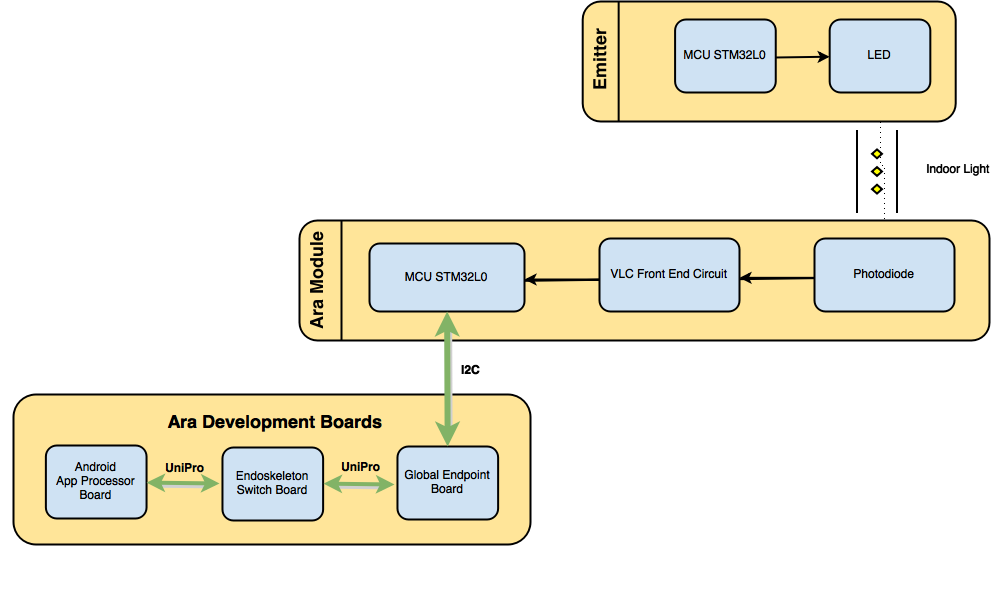
\includegraphics{Pictures/VLC-proposal-hard.png}
    }}
    \rule{35em}{0.5pt}
  \caption[Proposal hardware implementation]{Proposal hardware implementation}
  \label{fig:RxCircuit}
\end{figure}


%----------------------------------------------------------------------------------------
%	HARDWARE
%----------------------------------------------------------------------------------------

\section{VLC Contribution}

Our approach would demonstrate a new VLC usage and possibility carrying an improved among of data the the user smartphone. Even if we follow IEEE 802.15.7 standard recommendation for PHY mode , we propose to combine OOK modulation with 4B6B coding, in order to improve emitted light power, avoid flickering, and improve the number of bit per symbol. In addition, we increase the emitter clock rate, up to 560kHz.

\begin{figure}[htbp]
  \centering
    \makebox[\textwidth][c]{
      \scalebox{0.35}{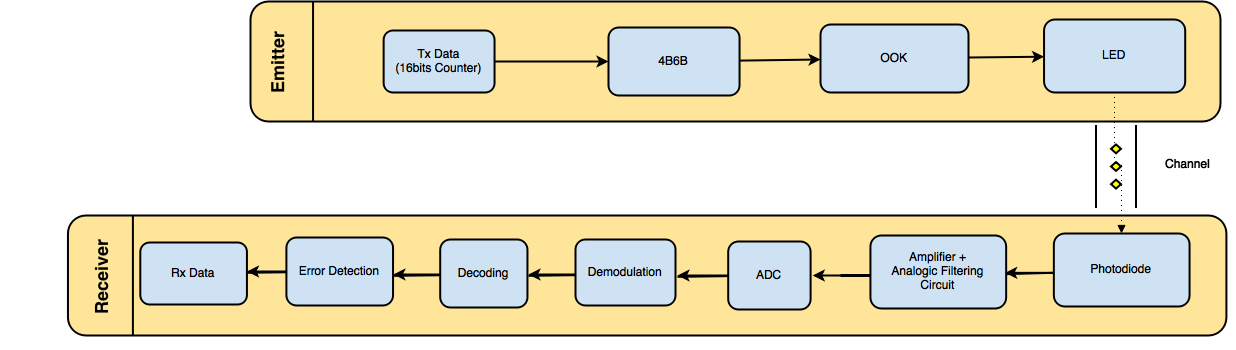
\includegraphics{Pictures/VLC-proposal.png}
    }}
    \rule{35em}{0.5pt}
  \caption[VLC system proposal]{VLC system proposal}
  \label{fig:RxCircuit}
\end{figure}


